% (C) 2016 Jean Nassar. Some Rights Reserved
% Except where otherwise noted, this work is licensed under the Creative Commons Attribution-ShareAlike License, version 4
% Background
\chapter{Background}
\label{ch:background}

\section{Prior work}
Several methods to show a robotic avatar in a virtual environment were proposed.

Nielsen et al. presented an interface in which a \gls{not:3d} model of the robot, a video stream from a mounted camera, a map, and pose information, were combined in a mixed-reality display.\cite{nielsen2007}
Kelly et al. extended the concept to an outdoor environment, and succeeded in making their system work in various low-throughput situations.\cite{kelly2011}

However, most methods require many sensors, which add expense and weight to the vehicle.

\section{Teleoperation System Using Past Image Records}
Shiroma et al. introduced \gls{spir}, a past-image view technique for mobile robots.\cite{shiroma2004}
This technology enabled the operator to ascertain the position and orientation of the robot with respect to its environment from a third-person (bird's-eye view) perspective using only the camera and position and pose information.

\begin{figure}[h]
  \centering
  \begin{subfigure}[b]{0.45\textwidth}
    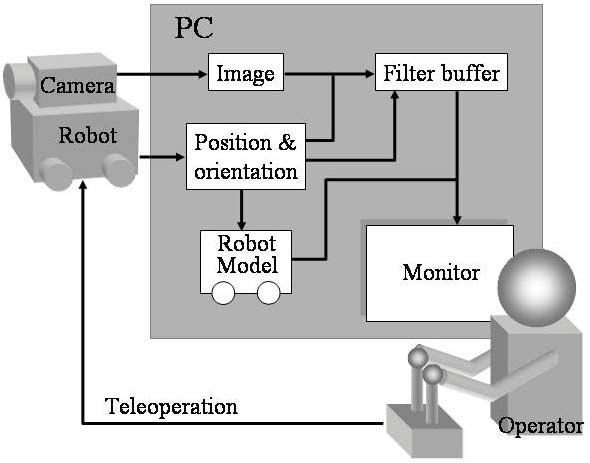
\includegraphics[width=\textwidth]{spir_system_overview}
  \end{subfigure}
  \hfill
  \begin{subfigure}[b]{0.45\textwidth}
    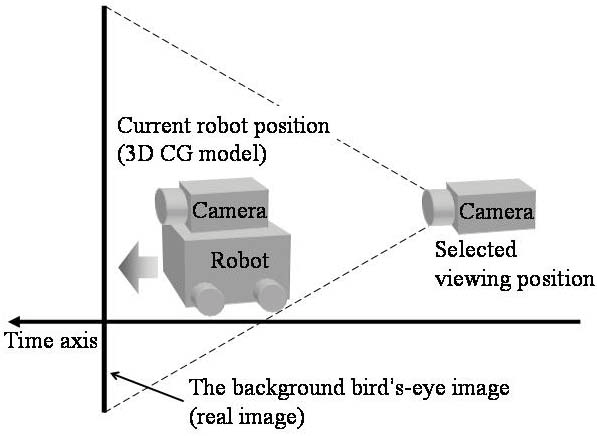
\includegraphics[width=\textwidth]{spir_birdseye}
  \end{subfigure}
  \caption{System overview of Past-Image View.\cite{shiroma2004}}
  \label{fig:spir_system_overview}
\end{figure}

Images taken by a raised camera were saved in a buffer along with their position and the time at which they were taken.
No images are stored while the robot is not moving.
Three evaluation functions were proposed to select an optimal image to use as the background:

\begin{description}
  \item [Fixed time delay:] uses images taken a certain period earlier.
  \item [Fixed distance:] uses images taken at approximately the given distance.
  \item [\Gls{fov} evaluation:] selects the closest image if the robot is in the field of view.
\end{description}

\begin{figure}[h]
  \centering
  \begin{subfigure}[b]{0.45\textwidth}
    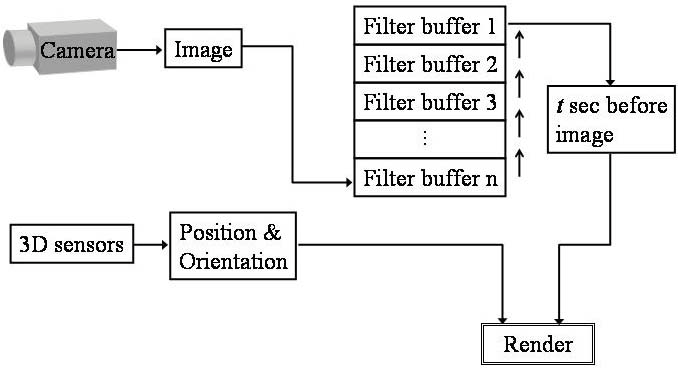
\includegraphics[width=\textwidth]{spir_time_delay}
    \caption{Fixed time delay algorithm.}
    \label{fig:spir_time_delay}
  \end{subfigure}
  \hfill
  \begin{subfigure}[b]{0.45\textwidth}
    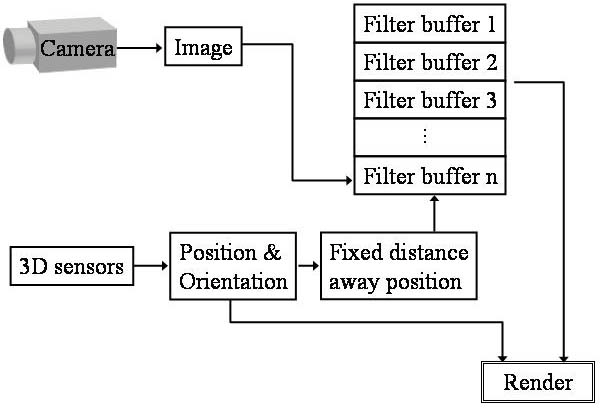
\includegraphics[width=\textwidth]{spir_fixed_distance}
    \caption{Fixed distance algorithm.}
    \label{fig:spir_fixed_distance}
  \end{subfigure}
  \caption{The naïve algorithms.\cite{shiroma2004}}
  \label{fig:spir_naive_algorithms}
\end{figure}

\Gls{fov} evaluation uses the fixed-distance algorithm as the base, but also calculates view and centreline distances, as well as the widths at the bottom and centre of the image.

\begin{figure}[h]
  \centering
  \begin{subfigure}[b]{0.3\textwidth}
    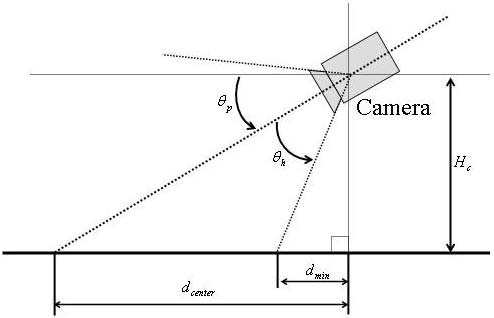
\includegraphics[width=\textwidth]{spir_fov_side_view}
    \caption{Side view.}
    \label{fig:spir_fov_side_view}
  \end{subfigure}
  \hfill
  \begin{subfigure}[b]{0.3\textwidth}
    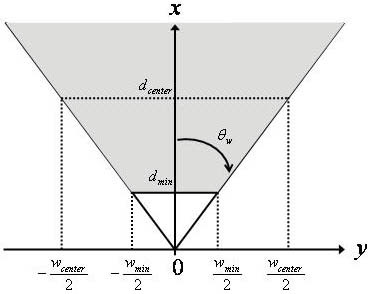
\includegraphics[width=\textwidth]{spir_fov_top_view}
    \caption{Top view.}
    \label{fig:spir_fov_top_view}
  \end{subfigure}
  \hfill
  \begin{subfigure}[b]{0.3\textwidth}
    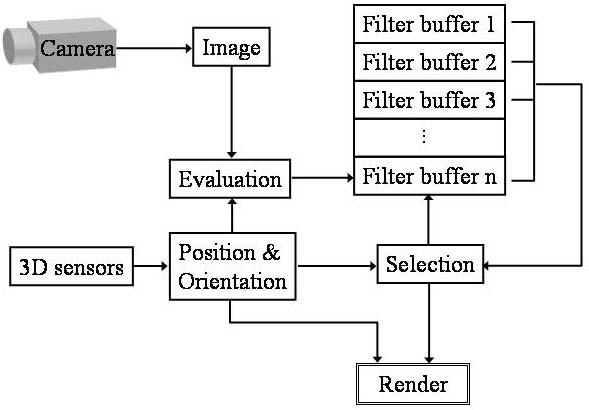
\includegraphics[width=\textwidth]{spir_fov}
    \caption{\Gls{fov} evaluation.}
    \label{fig:spir_fov_flowchart}
  \end{subfigure}
  \caption{\Gls{fov} evaluation algorithm.\cite{shiroma2004}}
  \label{fig:spir_fov}
\end{figure}

An optimal image was then found using an evaluation function considering several constraints, including \gls{fov} and the relative positions of the camera and robot.
The latest image is used if no good solution can be found.

If the bandwidth is low, old images can be reused, updated by an array of position data sent at a higher speed than the video.

\subsection{Further development}
Sugimoto et al. demonstrated the effectiveness of \gls{spir} with user experiments.\cite{sugimoto2005}
Ito et al. decreased choppiness by proposing wider \glspl{fov}, and zooming into the background and model as the robot went further into the image plane.\cite{ito2008}
They also experimented with adding trajectory forecasting with unmanned ground vehicles.

\begin{figure}[h]
  \centering
  \begin{subfigure}[b]{0.45\textwidth}
    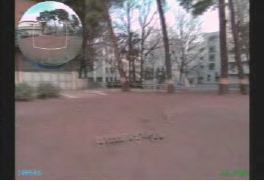
\includegraphics[width=\textwidth]{zoom_live}
  \end{subfigure}
  \hfill
  \begin{subfigure}[b]{0.45\textwidth}
    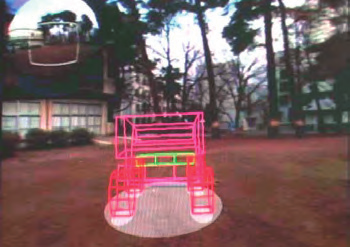
\includegraphics[width=\textwidth]{zoom_combined}
  \end{subfigure}
  \caption{Zoom with bird's-eye view synthesis.\cite{ito2008}}
  \label{fig:zoom_results}
\end{figure}

Murata et al. extended the concept to \gls{not:3d} when they applied it to mobile manipulators.\cite{murata2014}
They showed a significant decrease in operators' position error in the vertical direction with a similar error in the longitudinal direction.

\begin{figure}[h]
  \centering
  \begin{subfigure}[b]{0.45\textwidth}
    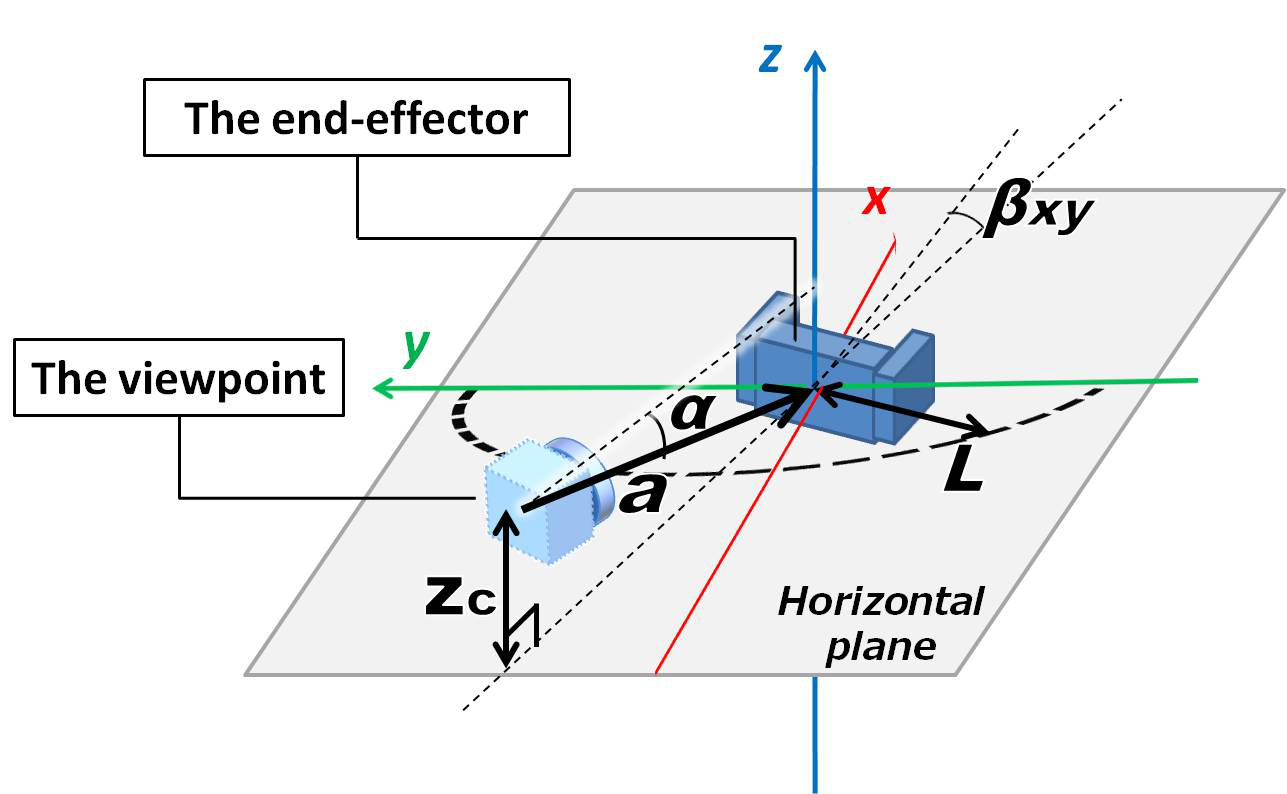
\includegraphics[width=\textwidth]{manip_overview}
    \caption{Geometric relationships.}
  \end{subfigure}
  \hfill
  \begin{subfigure}[b]{0.45\textwidth}
    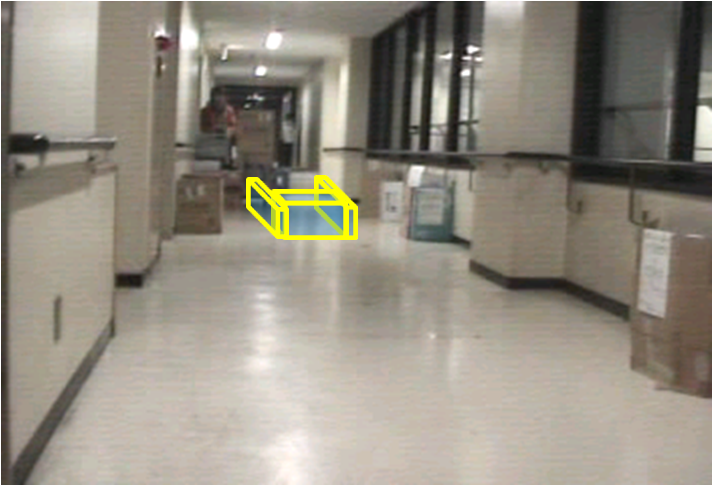
\includegraphics[width=\textwidth]{manip_result}
    \caption{Basic display concept.}
  \end{subfigure}
  \caption{\gls{spir} for a mobile manipulator.\cite{murata2014}}
  \label{fig:manip_results}
\end{figure}

\section{Problems of applying SPIR to quadrotors}
When a quadrotor flies forwards, the craft pitches down.
For cameras which do not offer gimballing or a wide \gls{fov}, though, this means that the horizon could go out of frame.
As a result, older video would need to be used, which would likely be from a longer distance.
If the drone turns while going forward, the only usable images might be the live ones.

One potential mitigating factor would be to set a maximum pitch angle, though that would limit the speed of the drone.
Even so, during straight and level flight, an operator would only be able to see the drone from behind, unless an elevated camera is attached.

Another possible solution would be to tilt the camera upwards.
This would limit the amount of ground it would see during a hover.
In addition, it would cause the camera to be pointing at the sky while the drone is outdoors and moving backwards, removing potential reference points.

Finally, localization can be difficult too.
Even outdoors, \gls{gps} only tends to be accurate to within a few metres, which is much larger than the widths of most drones.
While estimates of acceleration can be obtained by modelling the motor outputs and using built-in accelerometers and gyroscopes, there is often drift from wind, as well as significant vibration even during hovering.
Integrating acceleration twice to obtain position would cause exponentially increasing drift.

External sources could be used to reduce the error, such as motion capture cameras if indoors, binocular cameras, visual odometry, \gls{gps}, or \gls{slam}.
That might require the use of more additional tools, such as ultrasonic distance sensors or laser range finders.
An \gls{ekf} could then be used to estimate the best location and minimize drift.
However, that is beyond the scope of this research.

Some \gls{slam} algorithms, such as \gls{ptam} and \gls{rtslam}, are able to use monocular cameras, but rotation on the spot often causes them to lose keypoints, making them a bad choice for drones.

\section{Proposal}
My proposal goes here.

% SPIRIT
\chapter{Superimposed Past Image Records Implemented for Teleoperation}
\label{ch:spirit}

\section{System overview}
  There are six main parts to the project:

  \begin{itemize}
    \item An operator-controlled gamepad sends commands to the drone.
    \item The pose, consisting of the position and orientation of the drone, is calculated by a motion capture system and relayed to the operating station.
    \item The drone streams video at 30\,Hz, which is downsampled to 2\,Hz to simulate \gls{los} conditions.
    \item The 2\,Hz video feed is shown to the operator without modification.
    \item All received images are also stored in a chronological array.
	  When a new pose is received, it is checked against frames in reverse order using an evaluation function.
    \item The frame with the lowest score is selected, and has the current pose rendered onto it to show to the operator.
  \end{itemize}

  The past image selector and the visualization system are discussed in separate sections.

  \subsection{Environment}
    The operating station runs \gls{ros} Jade on Ubuntu 15.04.
    A separate computer is connected to the lab's motion capture system.
    Both computers are connected to each other via ethernet.

    The drone connects to the operating station by acting as a Wifi access point.
    Communication with the drone is achieved using the Simon Fraser University Autonomy Lab's \verb|ardrone_autonomy| package.

  \subsection{Control}
    The computer receives operator input from an off-the-shelf console gamepad, and forwards it to the drone.
    A \gls{gui} was taken from the \verb|drone_gui| node of \verb|tum_ardrone|, written by the Computer Vision group at the Technische Universität München, and controller interaction used the \verb|joy| package.

  \subsection{Video}
    A live, 30\,Hz feed is received from the drone.
    Every fifteenth frame is then selected in order to drop the frequency to 2\,Hz.
    Both feeds are published for other nodes, and the slow video is displayed to the operator during tests.

  \subsection{Pose}
    Optitrack's \emph{Motive} software is used to collect data on the position and orientation of the drone.
    Four infrared markers are set onto the top of the drone, and the Optitrack infrared cameras are connected to the motion capture computer.
    The markers forming the drone are defined as a rigid body, and the resulting centre is adjusted to align with the camera.

    The motion capture system sends the data to the operating station, where it is interpreted by the \verb|mocap_optitrack| package before being published to the rest of the system.
    In the process, eulerian coordinates are changed into quaternions.

    The pose data is followed to ascertain the status of the tracking.
    If the motion capture system is unable to determine the pose of the drone, whether by occlusion of a marker or a venture outside of the field of view of the cameras, the values would stop updating.
    In that case, a flag is set that can be used by other nodes.
    Losing tracking also gives a visual and an aural warning to notify the operator, as the visualization system would not be showing the correct information.

    One method, which was not used, was \verb|ardrone_autonomy|'s ability to obtain drone odometry from the bottom-facing camera, \gls{imu}, altimiter, and barometer.
    The ground velocity is calculated using integration of acceleration as well as optical flow.
    While the final result proved to be accurate, the calculations required were slow in a tight loop, so it was discarded in favour of the motion capture system.

\section{The past image selector}
  Each new image that arrives while the pose is being tracked is automatically packaged into a \texttt{Frame} object containing the time it was taken, as well as the position and orientation of the drone at that time.
  These \texttt{Frame}s are then stored in a chronological list.

  When a new valid pose arrives, it is checked against the frames in reverse order using an evaluation function.
  The \texttt{Frame} with the lowest score is published for use by the visualization system.

  However, while the pose was sampled at 30\,Hz (every 0.33\,s), each iteration of the some evaluation functions requires up to 0.3\,ms to run.
  As a result, when about a hundred frames are collected, a substantial lag in image selection can be detected.
  For those algorithms, only one hundred frames were selected by skipping a certain number each time, while still keeping a good representation of the entire course of the drone's flight.
  This allows each loop to run its course before the next pose is received.

  \subsection{Chronological list}

  \subsection{Evaluation functions}
    The simplest evaluation function for past image view is one with constant time delay.
    One can quickly find a frame with a specific age by doing a binary search on a chronologically-ordered array.
    However, it has this and that problem...
     % \subsubsection{Simple evaluation functions}
     % \subsubsection{Final evaluation function}


\section{Rendering}
  \subsection{OpenGL}

% Experiments
\chapter{Experiments}
\label{ch:experiments}
\section{Objectives}
  \subsection{Accuracy}
  \subsection{Completion speed}
  \subsection{Rate of improvement}
\section{Design}
\section{Participants}
\section{Task description}
\section{Experiment setup}
\section{Evaluation method}
  \subsection{Completion standards}
  \subsection{Subjective questioinnaire}

% Results
\chapter{Results}
\label{ch:results}
\section{Results}
  \subsection{Time}
  \subsection{Speed}
  \subsection{Stoppage}
  \subsection{Error rate}
  \subsection{Workload}
  \subsection{Interview}
\section{Analysis}
\begin{figure}[h]
  \centering
  \input{img/binomial_factor_posterior.pgf}
  \caption{Analysis of binomial distribution. A Jeffreys noninformative prior ($\alpha = \beta = 0.5$) is used. The posterior distribution considers twenty successes out of thirty trials.}
  \label{fig:binom}
\end{figure}
\section{Discussion}

% Conclusions
\chapter{Conclusions}
\label{ch:conclusion}
\section{Conclusions}
\section{Future work}
\begin{itemize}
  \item Zooming
  \item Tilting
  \item Expand buffer using n-tree for quick selection
\end{itemize}
